\subsection{Architektur eines Expertensystems}\label{subsec:Architektur}
Beierle und Kern-Isberner betonen, dass die Trennung zwischen der Darstellung des Wissens (Wissensbasis) und der Wissensverarbeitung (Wissensverarbeitungskomponente) der wichtigste Aspekt eines Wissensbasierten Systems ist. \cite[S.11]{beierle2014}. Die Wissensbasis kann man sich als eine Art Datenstruktur vorstellen, in der das ben�tigte Wissen gespeichert wird. Die Wissensverarbeitungskomponente umfasst eine Menge von anwendungsunabh�ngigen Algorithmen, die mithilfe der Wissensbasis eine L�sung f�r ein gegebenes Problem erarbeiten. Somit stehen die Wissensbasis und die Wissensverarbeitungskomponente in einer engen Beziehung zueinander \cite[S.18]{kurbel1992}.\\
Allgemein umfasst ein Expertensystem folgende Bestandteile \cite[S.75]{greer2010}:
\begin{itemize}
\item \textit{Wissensbasis}, die Expertenwissen in Form von Fakten in einer bestimmten Sprache speichert sowie Regeln zur Wissensorganisation beinhaltet.
\item \textit{Inferenzmaschine}, die unter Ber�cksichtigung des zugrunde liegenden Wissensbedarfs die Wissensbasis
durchsucht bis das System einen Probleml�sungsvorschlag erarbeitet hat oder herausfindet, dass keiner existiert.
\item \textit{Dialogkomponente}, die eine Schnittstelle zwischen dem Nutzer und dem System darstellt. 
\item \textit{Erkl�rungskomponente}, die dem Benutzer erl�utert, warum und auf welche Weise eine bestimmte L�sung gefunden bzw. nicht gefunden wurde \cite[S.126]{haun2000}.
\item \textit{Wissensakquisitionskomponente}, die den Entwickler des Expertensystems bei der Erweiterung, �nderung und Wartung der Wissensbasis unterst�tzt.
\end{itemize}
Laut Tecuci stellen Wissensbasis und Inferenzmaschine grundlegende Bestandteile eines Expertensystems dar und bilden damit den Kern des Expertensystems \cite[S.1444]{tecuci1992}. Dialogkomponente, Erkl�rungskomponente und Wissensakquisitionskomponente geh�ren zur sogenannten Schale und sind f�r die Kommunikation zwischen dem Systemverwalter und dem Nutzer zust�ndig (siehe Abbildung \ref{expertensystem_haun}). 
\begin{figure}[H] 
	\centering
	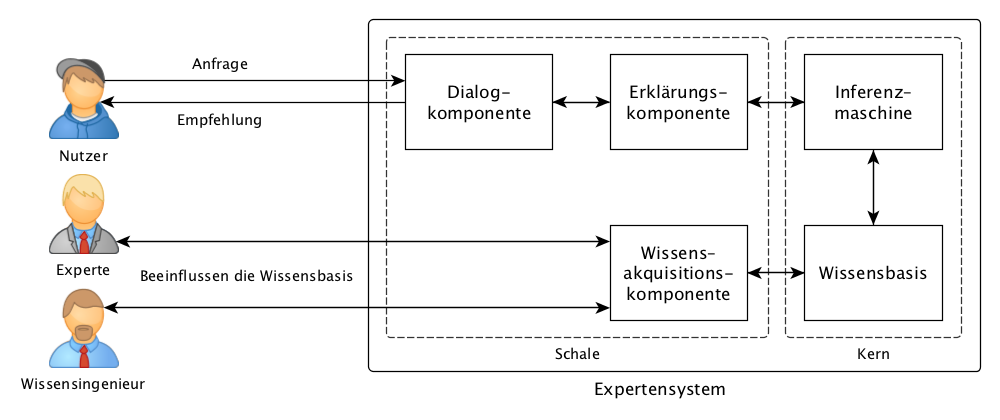
\includegraphics[width=1.0\textwidth]{images/expertensystem_haun.png}
	\caption{Architektur eines Expertensystems nach Haun, \cite[S.126]{haun2000}}
	\label{expertensystem_haun}
\end{figure}
Im Hinblick auf die Interaktion gibt es drei Gruppen, die mit dem Expertensystem interagieren: 
\begin{itemize}
\item \textit{Nutzer}, der das Expertensystem zum L�sen eines Problems benutzt und mit der Dialogkomponente kommuniziert. Der Wissensingenieur und der Experte k�nnen ebenso als Nutzer auftreten \cite[S.758]{wachsmuth1993}.
\item \textit{Wissensingenieur}, der sich mit dem Aufbau und Wartung der Wissensbasis besch�ftigt. Unter anderem ist Wissensmodellierung ein wichtiger Aufgabenbereich eines Wissensingenieurs \cite[S.742]{wachsmuth1993}.
\item \textit{Experte}, der �ber spezifisches Erfahrungswissen verf�gt, das f�r das Expertensystem relevant ist.
\end{itemize}
Der Ablauf der Kommunikation zwischen dem Nutzer und dem Expertensystem sieht folgenderma�en aus: 
\begin{itemize}
\item Der Nutzer schickt eine Anfrage an die Dialogkomponente des Expertensystems.
\item Die Dialogkomponente �bermittelt die Anfrage an die Inferenzmaschine.
\item Die Inferenzmaschine erarbeitet eine L�sung f�r das gegebene Problem mittels der Wissensbasis und gibt das Ergebnis an die Dialogkomponente zur�ck. 
\item Anschlie�end teilt die Dialogkomponente dem Nutzer die L�sung des Problems mit. Falls keine L�sung zum Problem existiert, wird eine entsprechende Fehlermeldung angezeigt.
\end{itemize}
Auf der anderen Seite k�nnen die Inhalte der Wissensbasis von einem Wissensingenieur mithilfe der Wissensakquisitionskomponente beeinflusst werden. Der Wissenserwerb durch den Wissensingenieur ist die verbreitetste Vorgehensweise, neue Daten f�r ein wissensbasiertes System zu erschlie�en. Meistens handelt es sich um ein Interview zwischen dem Wissensingenieur und dem Experten \cite[S.76]{greer2010}, \cite[S.210]{fujihara1997}. Neben dem Interview kann der Wissensingenieur eine Recherche der verf�gbaren Wissensquellen wie Text, technische Zeichnungen oder Web-Ressourcen durchf�hren. Anschlie�end werden die Daten vom Wissensingenieur formalisiert und in die Wissensbasis gespeichert. \\
Die Wissensbasis kann in einigen F�llen von einem fachlichen Experten beeinflusst werden. Daf�r ist eine geeignete Expertenschnittstelle innerhalb der Wissensakquisitionskomponente notwendig, die den Experten erm�glicht, ihr Erfahrungswissen selbst zu formalisieren und gegebenenfalls zu warten \cite[S.743]{wachsmuth1993}. Die �berpr�fung des Dateninputs ist ebenfalls die Aufgabe der Wissensakquisitionskomponente. Dies kann mittels Durchf�hrung automatisierten Tests bei jeder �nderungsanfrage erfolgen, um die Konsistenz der Wissensbasis zu gew�hrleisten \cite[S.743]{wachsmuth1993}.\\
Um ein geeignetes Konzept der automatisierten Datenerfassung zu entwickeln, ist ein grundlegendes Verst�ndnis von der Struktur und Funktionsweise der Wissensbasis sowie der Wissensakquisitionskomponente erforderlich. Im weiteren Verlauf der Arbeit werden die Erkenntnisse �ber die Wissensbasis und die Wissensakquisitionskomponente erl�utert, die in der Forschung von Expertensystemen entstanden sind.
